%%%%%%%%%%%%%%%%%%%%%%%%%%%%%%%%%%%%%%%%%%%%%%%%%%%%%%%%%%%%%%%%
% Sablona pro zaverecnou zpravu k semestralni praci z BI-ZUM
% Kódování dokumentu: UTF8
% Verze: 1.0 (2013-01-28)
% Autor: Ing. Martin Šlapák
%%%%%%%%%%%%%%%%%%%%%%%%%%%%%%%%%%%%%%%%%%%%%%%%%%%%%%%%%%%%%%%%
%
% NEUPRAVUJTE PROSIM PARAMETRY DOKUMENTU, JAKO OKRAJE CI PISMO!
%
%%%%%%%%%%%%%%%%%%%%%%%%%%%%%%%%%%%%%%%%%%%%%%%%%%%%%%%%%%%%%%%%
%
% Celkova delka zpravy nesmi presahnout 1 stranu A4, vyjadrujte 
% se strucne, jasne a vecne - zadne omacky a slovni vata. Diky!
% Neprehazujte ani poradi sekci.
%
%%%%%%%%%%%%%%%%%%%%%%%%%%%%%%%%%%%%%%%%%%%%%%%%%%%%%%%%%%%%%%%%
\documentclass[a4paper,10pt,twocolumn]{article}
\usepackage{lmodern}
\usepackage[czech]{babel}
\usepackage[T1]{fontenc}
\usepackage[utf8]{inputenc}
\usepackage{graphicx}
\usepackage{float}
\usepackage[top=0.5cm,bottom=2cm,left=1cm,right=1cm]{geometry}
%gobble sezere cisla stranek, takze nebudou zadna
\pagenumbering{gobble} 
\title{Zpráva k 1. domácímu úkolu z předmětu MI-PAA}
\date{\today}
%%%%%%%%%%%%%%%%%%%%%%%%%%%%%%%%%%%%%%%%%%%%%%%%%%%%%%%%%%%%%%%%
% tady nastavte své jméno a email
\author{Jan Sokol \\ sokolja2@fit.cvut.cz}
%%%%%%%%%%%%%%%%%%%%%%%%%%%%%%%%%%%%%%%%%%%%%%%%%%%%%%%%%%%%%%%%
\begin{document}
\maketitle
%%%%%%%%%%%%%%%%%%%%%%%%%%%%%%%%%%%%%%%%%%%%%%%%%%%%%%%%%%%%%%%%
\begin{abstract}
Úkolem bylo nalézt řešení 0/1 problému batohu hrubou silou (tj. nalezení skutečného optimuma). Dále bylo třeba zkušebních datech pozorovat závislost výpočetního času na n (kde n je počet věcí v batohu). Druhou částí ukolu naprogramování řešení problému batohu heuristikou podle poměru cena/váha. Na těchto datech bylo třeba pozorovat závislost výpočetního času na n, a také průměrnou a maximální relativní chybu (tj. zhoršení proti exaktní metodě) v závislosti na n.
% Zde shrňte v několika větách co jste dělali, jak jste to dělali, jakých výsledků jste dosáhli. Vypíchněte to nejzajímavější. Zkusili jste nějakou pokročilou techniku? Tady se s ní pochlubte a pak ji dále rozepište v patřičné sekci. Zkuste se vejít do 150 slov.
\end{abstract}

%%%%%%%%%%%%%%%%%%%%%%%%%%%%%%%%%%%%%%%%%%%%%%%%%%%%%%%%%%%%%%%%
\section{Parametry algoritmu, výběr jazyka}
Pro svou implementaci problému batohu jsem si vybral jazyk Python. Ačkoli to je jazyk interpretovaný a nečekal jsem závratné rychlosti výpočtů, mojím výběrem byl pro to, že jsem jazyk znal a pro jakýkolik koncept je pro mne nejrychlejší.

V případě hledání řešení hroubou silou jsem těžil z materiálů v přednáškách, tak i na internetu.

Při výpočtu heuristikou jsem vybral řazení dle snižující ceny. Poté jsem objekty do batohu přidával, dokud nebylo možné přidat další věc.


\section{Testovací Hardware}
Všechny testy byly prováděny na cloudové linuxové instanci v AWS, běžící na Red Hat Enterprise Linux 7. Velikost instance byla:
  2 Core CPU / 8 GB RAM, v názvosloví AWS \textbf{m4.large}.


\section{Měření výpočetního času}
Výpočet běhu funkce je řešen tak, že je spočten strojový čas před během funkce, a také po něm. Tyto časy jsou od sebe odečteny a je vrácen čas v ms.

   \begin{verbatim}
def timing(f):
    def wrap(*args):
        time1 = time.time()
        ret = f(*args)
        time2 = time.time()
        measured_time.append(
          {'type': f.__name__,
           'time': (time2-time1)*1000.0})
        return ret
    return wrap
   \end{verbatim}

\section{Brute force - závislost výpočetního času na n.}

Jak můžeme pozorovat u metody hrubé síly, složitost při velikosti batohu roste exponenciálně. Data, která byla využita pro vykreslení grafů jsou k dispozici v adresáři \textbf{report/data/} v souboru \textbf{all\_times.csv}.

\begin{figure}[H]
  \begin{center}
    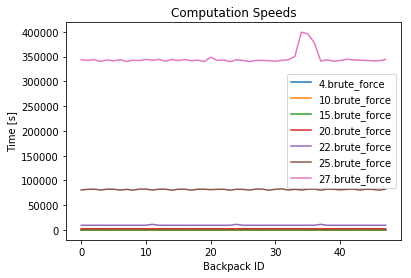
\includegraphics[height=6cm]{graphs/brute_force_speeds.png}
  \end{center}
  % \caption{Graf vývoje fitness}\label{fig1}
\end{figure}

\subsection{Heuristika - závislost výpočetního času na n.}

Díky tomu, že v metodě heuristiky pouze batoh sortíme a poté se snažíme přidat n objektů, můžeme říci, že složitost metody je lineární.

\begin{figure}[H]
  \begin{center}
    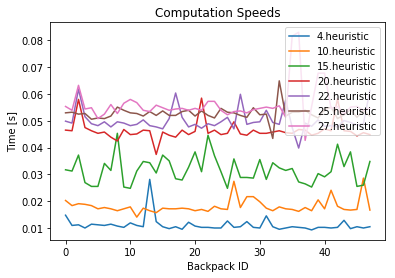
\includegraphics[height=6cm]{graphs/heuristic_speeds.png}
  \end{center}
  % \caption{Graf vývoje fitness}\label{fig1}
\end{figure}

\subsection{Průměrná a maximální relativní chyba}

Relativní chybu jsem počítal následovně:

$$  \epsilon = \frac{C(OPT)-C(APX)}{C(OPT)} $$ \\ kde \textbf{C(OPT)} je cena optima (získaného z referenčního řešení), \\
a \textbf{C(APX)} je cena přibližného řešení (vypočítaná funkcí heuristic).

Relativní chyby byly vypočítány jednotlivě pro všechny instance a poté zprůměrovány (nebo vybrána maximální hodnota) pro každou velikost batohu.
\begin{figure}[H]
  \begin{center}
    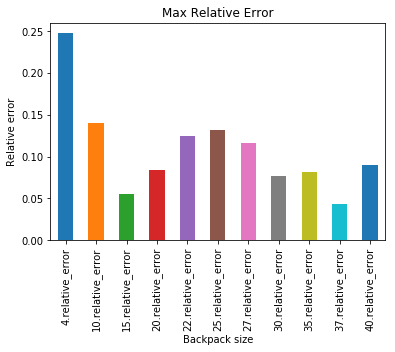
\includegraphics[height=6cm]{graphs/max_errors.png}
  \end{center}
  % \caption{Graf vývoje fitness}\label{fig1}
\end{figure}

\begin{figure}[H]
  \begin{center}
    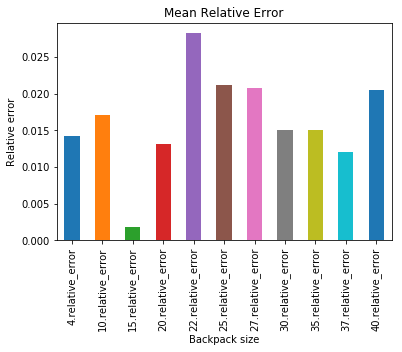
\includegraphics[height=6cm]{graphs/mean_errors.png}
  \end{center}
  % \caption{Graf vývoje fitness}\label{fig1}
\end{figure}

Ať už z maximálních, či průměrných relaticních chyb jsem nezpozoroval žádnou závislost relativní chyby na velikosti batohu. Data, která byla využita pro vykreslení grafů jsou k dispozici v adresáři \textbf{report/data/}.


% \section{Vývoj hodnoty fitness}
% Tady bychom \textbf{velmi rádi} viděli váš vlastní graf vývoje hodnoty fitness v průběhu všech generací. 
% % to H v hranate zavorce rike "put it HERE" vice zde:
% % http://en.wikibooks.org/wiki/LaTeX/Floats,_Figures_and_Captions#Figures
% % ps.: Graf ve vektorech nas potesi, at tam nevidime pixely. ;-)
% % jak na to, vas nauci na BI-TED, nebo se ptejte sluzebne starsich kolegu
% \begin{figure}[H]
%   \begin{center}
%     \includegraphics[width=3cm,height=3cm]{graph.png}
%   \end{center}
%   \caption{Graf vývoje fitness}\label{fig1}
% \end{figure}
% Nezapomeňte graf \ref{fig1} popsat slovy. Co je na něm vidět? Proč vypadá tak jak vypadá? Mohlo by se to vyvíjet lépe? Jak by se dal vývoj hodnoty fitness ovlivnit?

\section{Shrnutí a výsledky}

Pomocí metody hrubé síly jsem dosáhl pouze velikosti 27 - při velikosti bahohu již vypočtení testovacích dat trvalo více než 24 hodin. Díky tomu v grafech větší data pro měření rychlostí nejsou přiložena. 
Relativní chyba používá data z referenčního řešení, a díky tomu, že řešení heuristikou je mnohem rychlejší, než hrubou silou, proto data obsahuje pro všechny zadaná data.

Pro vytváření grafů bylo využito Python notebooku, který je přiložen v adresáři \textbf{report/}. Grafy jsou vykresleny pomocí knihovny \textbf{mathplotlib}.

% Tady okomentujte k čemu se váš evoluční algoritmus dopracoval, co se vám povedlo, co ne a jak by to šlo vylepšit. Jakého nejlepšího řešení se vám podařilo dosáhnout. Klidně i napište, co se vám na semestrální práci líbilo a taky co byste raději měli jinak. Uvítáme jakékoli nápady. 

% Pokud jste čerpali z nějaké literatury, měli byste ji řádně ocitovat.

% \textbf{A NEZAPOMEŇTE, ŽE SE MUSÍTE VEJÍT NA JEDNU A4! ;-)}

%%%%%%%%%%%%%%%%%%%%%%%%%%%%%%%%%%%%%%%%%%%%%%%%%%%%%%%%%%%%%%%%
% odtud dal to pak zakomentujte pomoci znaku procenta na zacatku radku
% \begin{center}
% \line(1,0){250}
% \end{center}

% \textbf{Pár poznámek pod čarou\ldots}
% \begin{itemize}
%   \item Zdroják této šablony je v kódování UTF8.
%   \item Neměňte prosím žádná nastavení dokumentu, okrajů, velikosti písma apod.
%   \item Nepřehazujte ani pořadí sekcí.
%   \item \textbf{Jak zprávu zkompilovat?} Použijte dvakrát (kvůli odkazům a referencím) tento příkaz:

%   \begin{verbatim}
%   pdflatex zdrojak-zpravy.tex
%   \end{verbatim}

%   Výsledkem bude \textbf{zdrojak-zpravy.pdf}. 

%   \item Pokud něco nepůjde, konzultujte na cvičeních BI-TED či se spolužáky. Cvičící BI-ZUM nebudou mít čas řešit detaily s {\LaTeX}em.
%   \item \textbf{Proč se sakra musím vejít na 1 A4?} Chceme, abyste si vyzkoušeli jak napsat to podstatné, vybrat to důležité, vyhnout se takové té textové vatě. Současně po vás nechceme psaní dlouhých esejí, raději svůj čas věnujte svým algoritmům. A taky, kdo má číst 5 stran napsaných \uv{protože to chtěj}. ;-)
%   \item TIP: Tuto zprávu může být reálné uplatnit i jako jeden z domácích úkolů na BI-TED. K tomu vás ale nenutíme a také počítejte s tím, že tam po vás mohou chtít další rozšíření dokumentu. \textbf{Ale zase: proč nezabít dvě mouchy jednou ranou?}
% \end{itemize}

\end{document}
